\section{Anhang}
	\subsection{Funktionen}
	
	%TODO siehe itemize TODO
	\textbf{TODO}
		\begin{itemize}
				\item Nat Skript S.237, Funktionen 9.2-9.5 ergänzen
				\item Anhang Kap. 3, 151-157 SigSys1 Fouriertransformierte
				\item Anhang Fouriertransformierte in Buch Elektrotechnik Europalehrmittelverlag, S323ff
		\end{itemize}
	
	
		\subsection{Rechteckimpuls}
		\begin{minipage}{0.2\textwidth}
			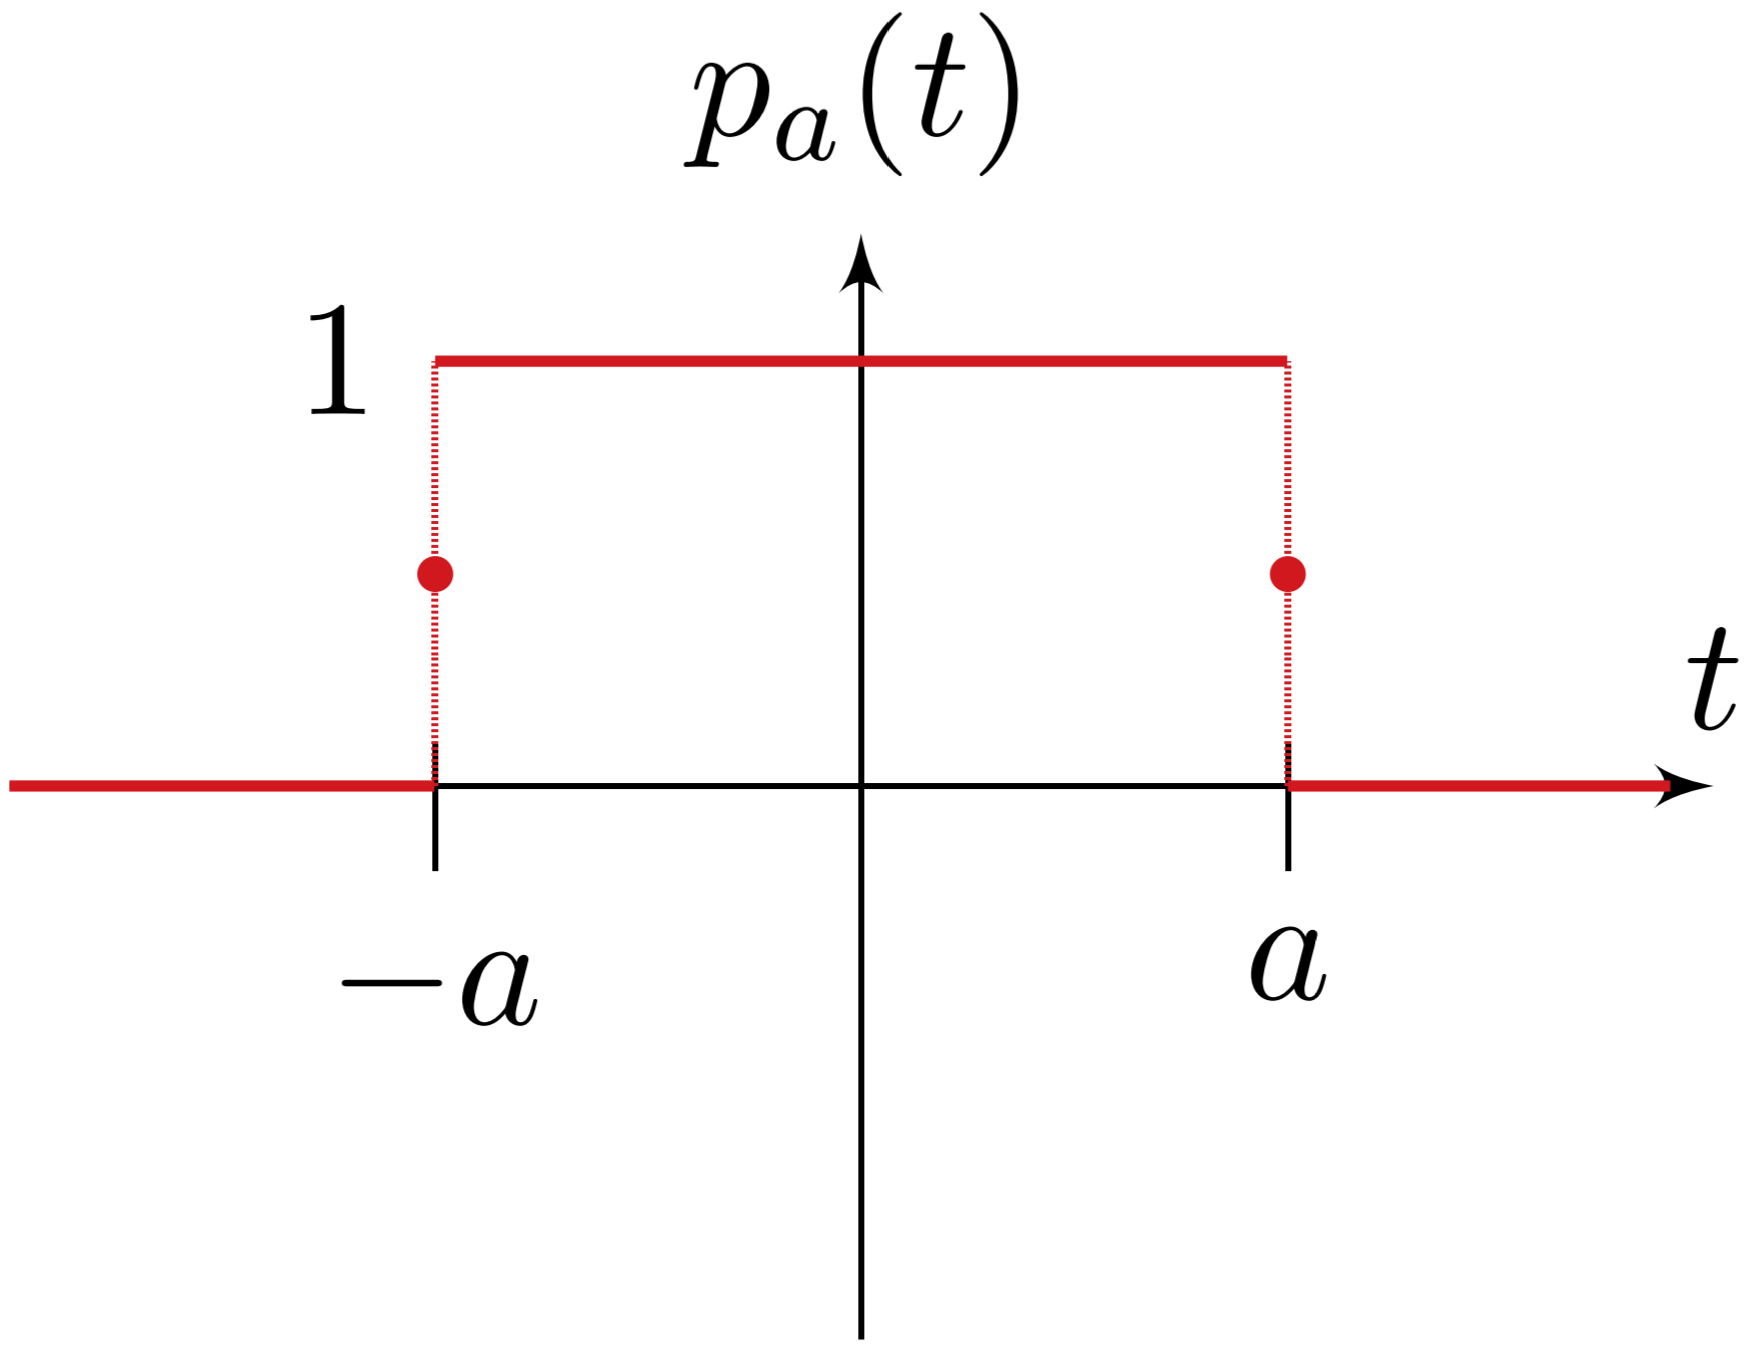
\includegraphics[width=\textwidth]{./bilder/funktionen/rechteckF.png}
		\end{minipage}
		\qquad
		\begin{minipage}{0.45\textwidth}
			$p_{a}(t)=\begin{cases}
			1 & |t|<a \\ 
			\frac{1}{2} & |t|=a \\ 
			0 & |t|>a
			\end{cases}$
		\end{minipage}
		\qquad
		\begin{minipage}{0.25\textwidth}						
			%
		\end{minipage}
		
		\subsection{Rampenfunktion}
		\begin{minipage}{0.2\textwidth}
			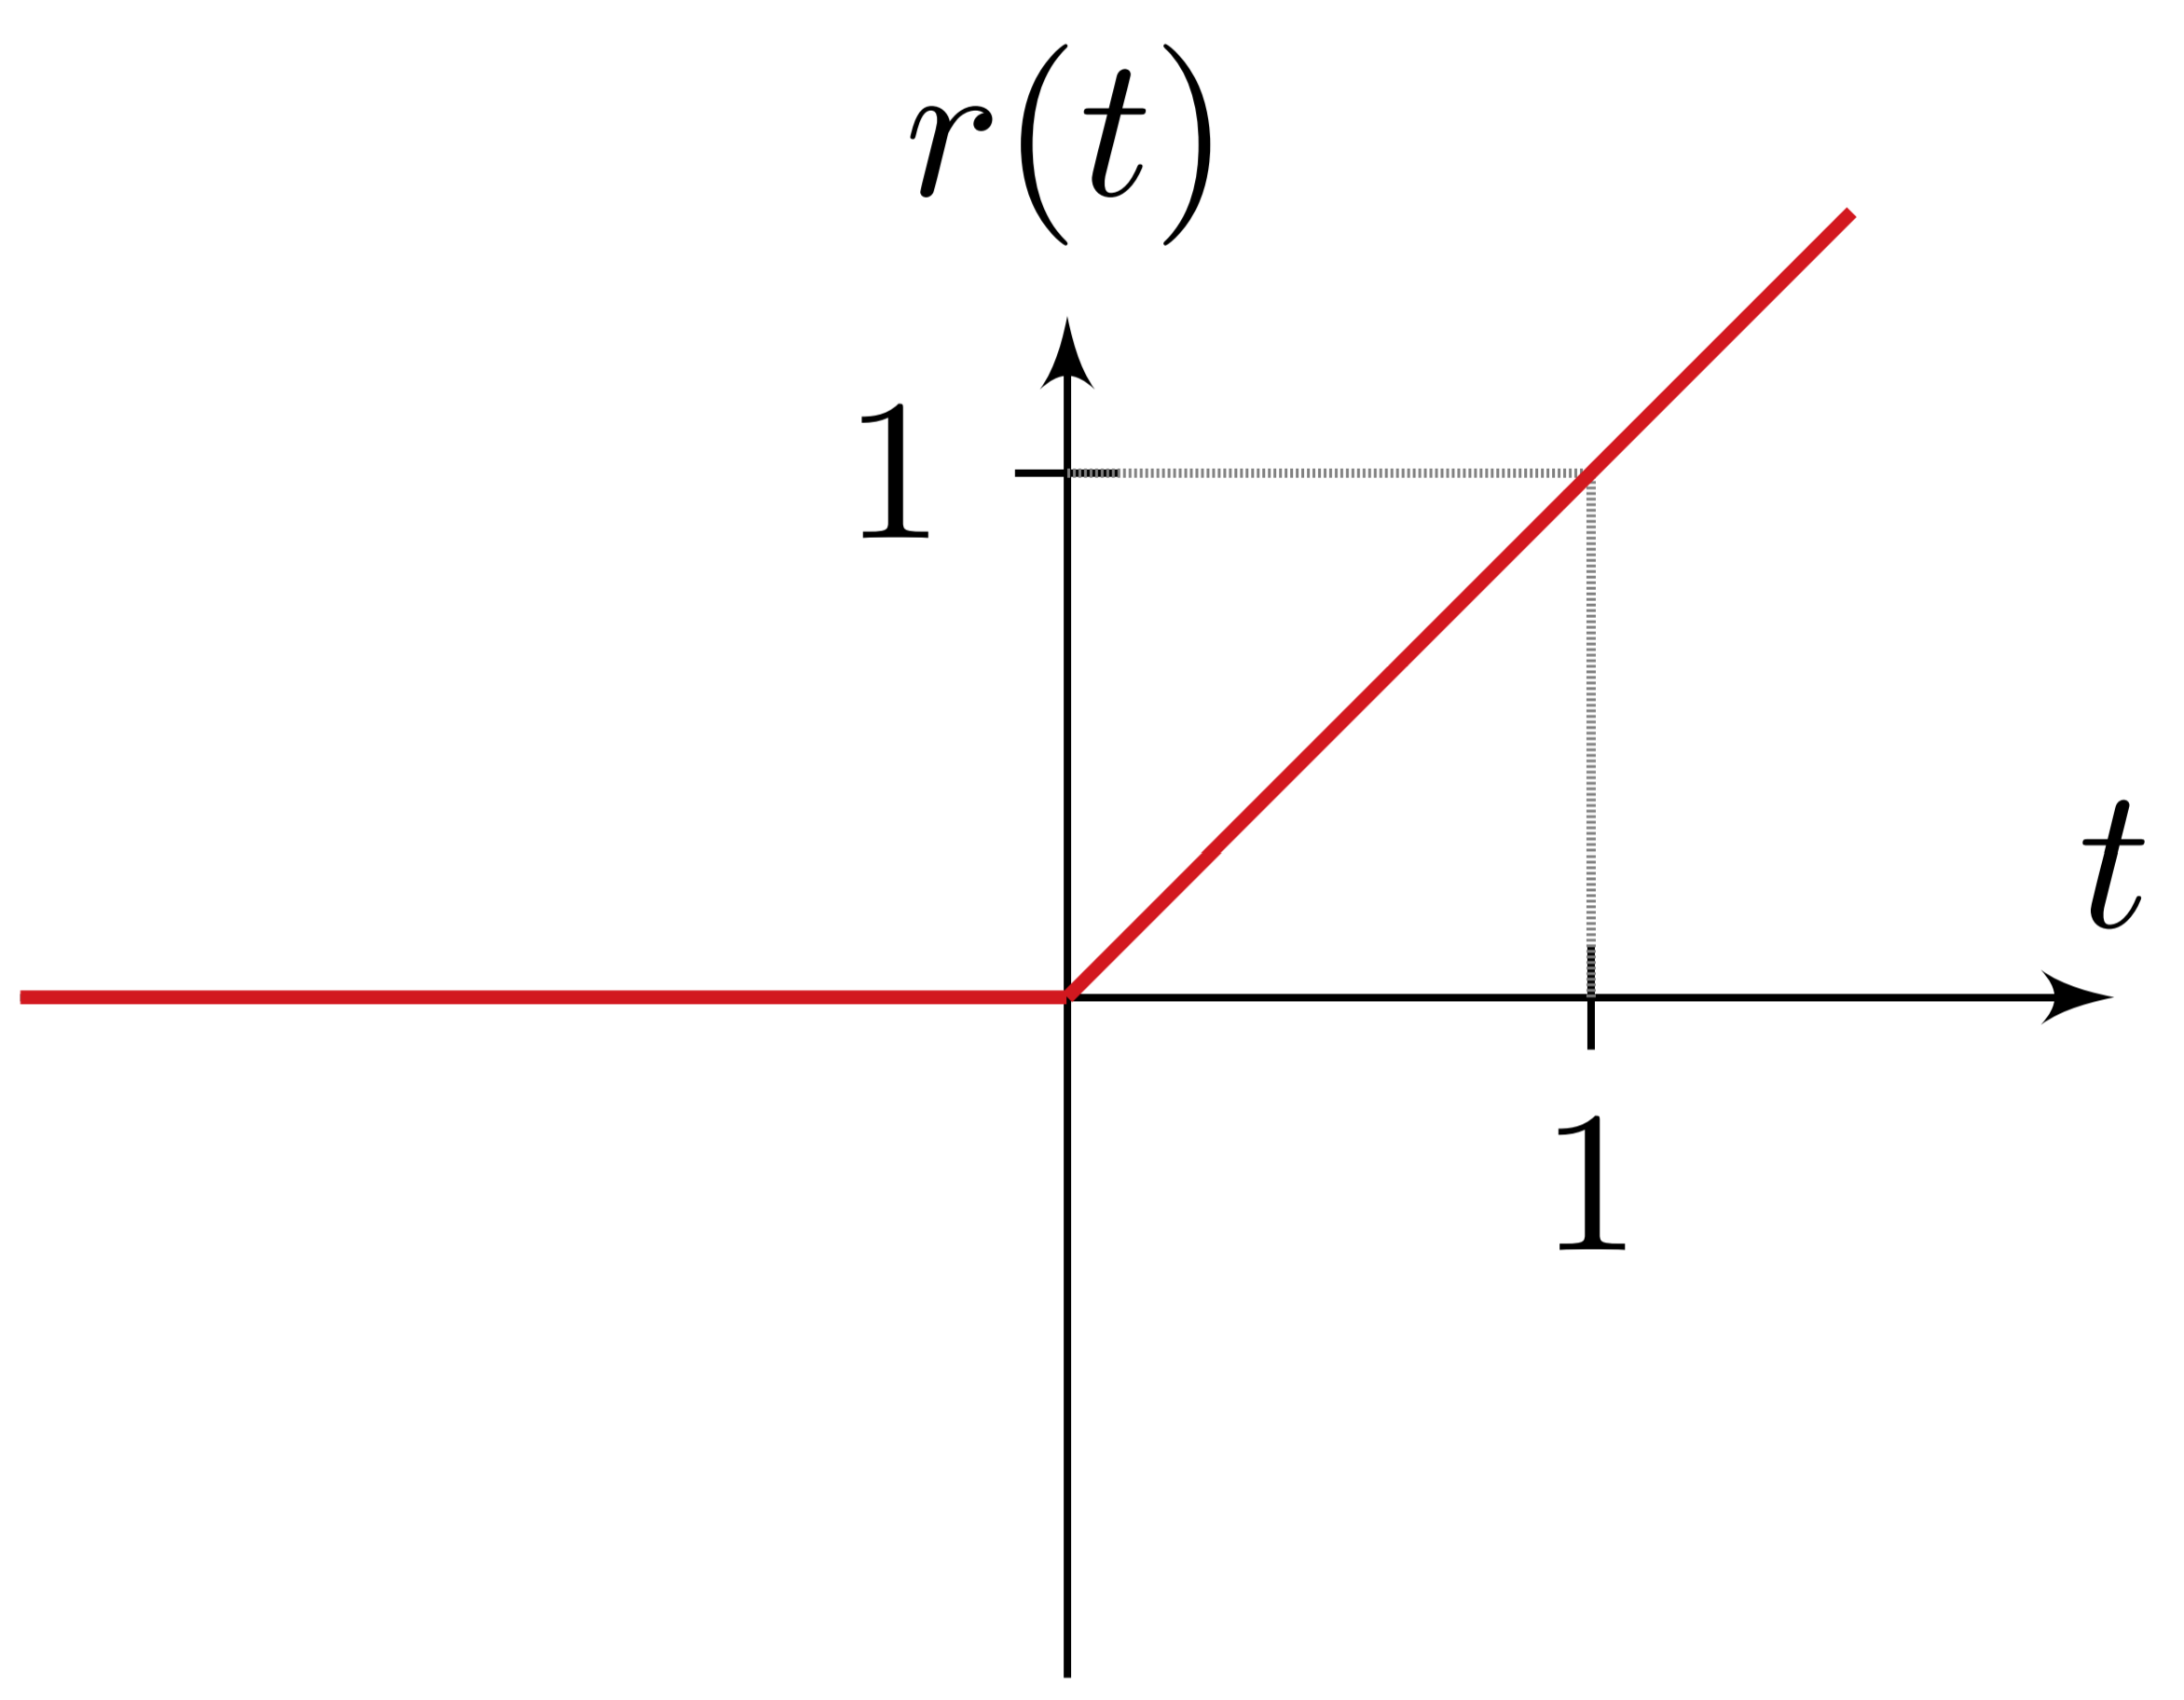
\includegraphics[width=\textwidth]{./bilder/funktionen/rampenF.png}
		\end{minipage}
		\qquad
		\begin{minipage}{0.45\textwidth}
			$r(t)=\begin{cases}
			{0} & {t \leq 0} \\ 
			{t} & {t>0}
			\end{cases}$
		\end{minipage}
		\qquad
		\begin{minipage}{0.25\textwidth}						
			%
		\end{minipage}		
		
		\subsection{Dreieckimpuls}
		\begin{minipage}{0.2\textwidth}
			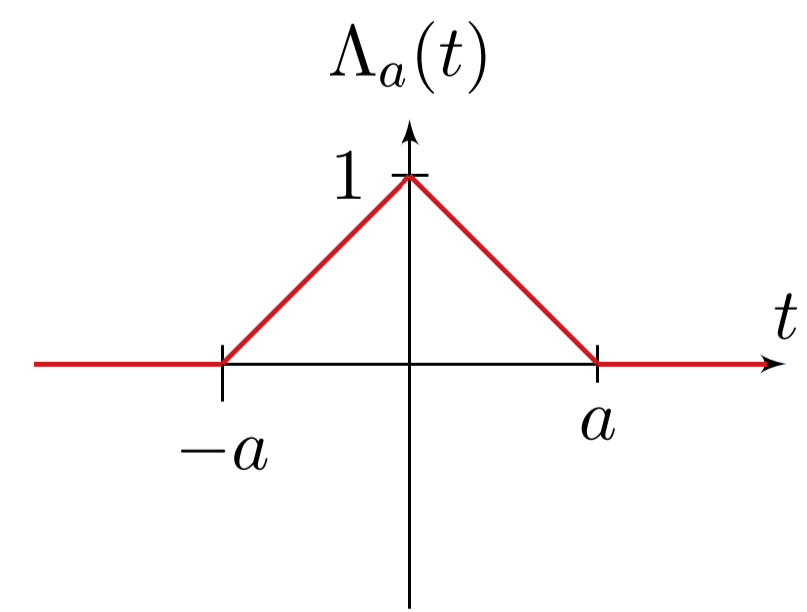
\includegraphics[width=\textwidth]{./bilder/funktionen/dreieckF.png}
		\end{minipage}
		\qquad
		\begin{minipage}{0.45\textwidth}
			$\Lambda_{a}(t)=\begin{cases}{1-\frac{|t|}{a}} & {t<a} \\ {0} & {|t| \geq a}\end{cases}$
		\end{minipage}
		\qquad
		\begin{minipage}{0.25\textwidth}						
			%
		\end{minipage}
		
		
		\subsection{Sinc-Funktion}
		\begin{minipage}{0.2\textwidth}
			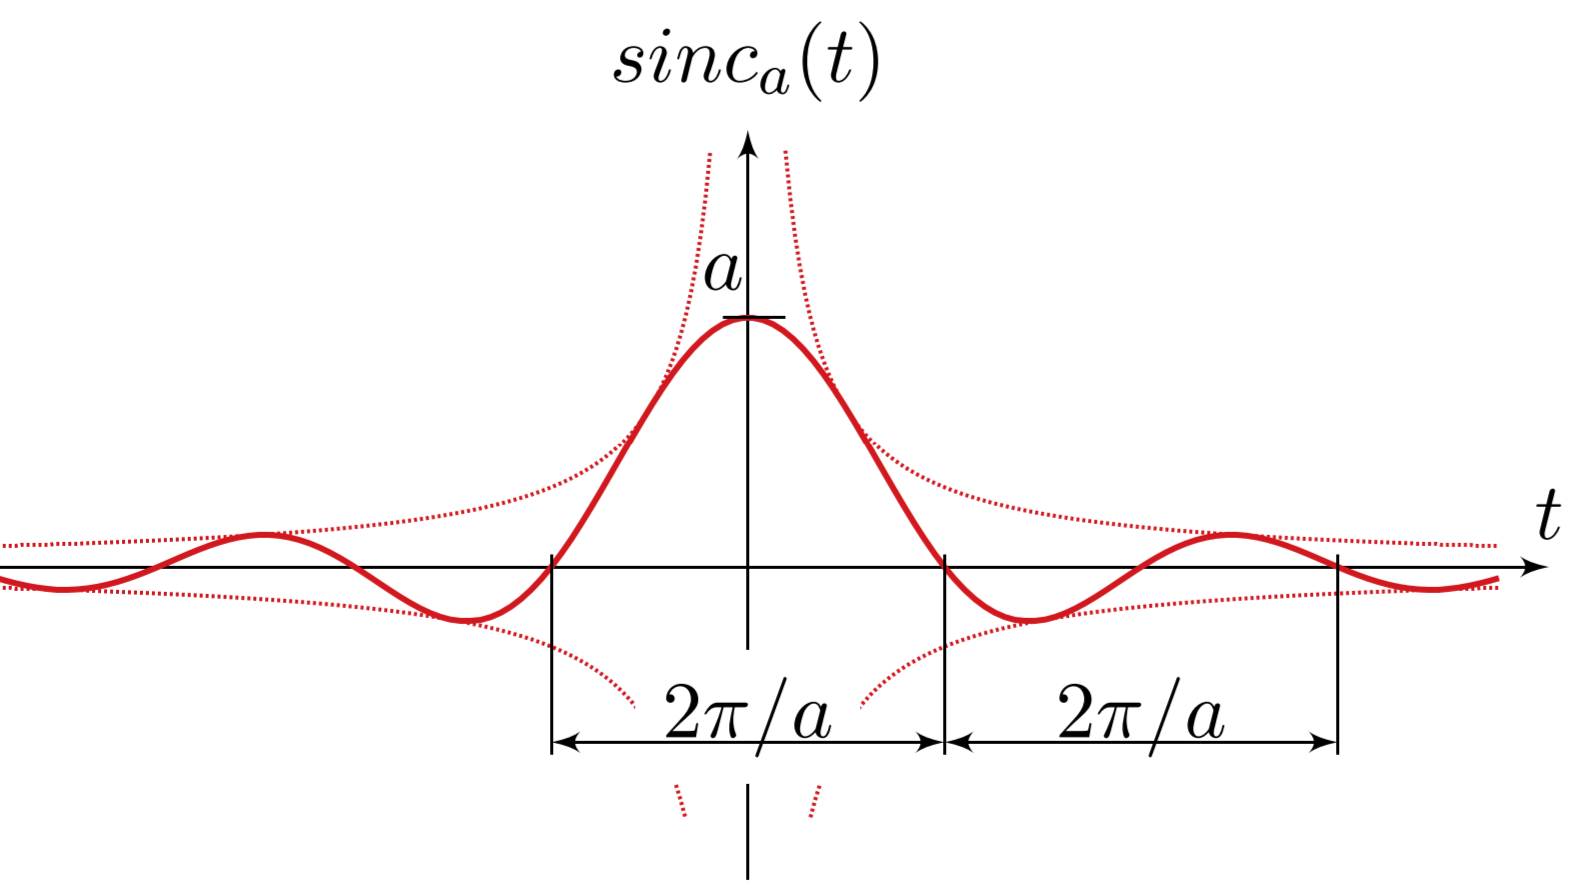
\includegraphics[width=\textwidth]{./bilder/funktionen/sincF.png}
		\end{minipage}
		\qquad
		\begin{minipage}{0.45\textwidth}
			\begin{math}
				\begin{aligned}
					\operatorname{sinc}_{a}(t) &= \frac{\sin (a t)}{t} \\
					\operatorname{sinc}(a t) &= \frac{\sin (a t)}{a t}
				\end{aligned}
			\end{math}
		\end{minipage}
		\qquad
		\begin{minipage}{0.25\textwidth}						
			%
		\end{minipage}\\
	
	
	